\documentclass{beamer}
\usetheme{Madrid}

%Packages BEGIN
\usepackage{amsmath}
\usepackage{physics}
\usepackage{hyperref} 
\usepackage{mathtools} 

%Packages END

% Chinese settings start
\usepackage{xeCJK} % use this package to set Chinese and English font separately
\setCJKmainfont{Noto Serif CJK TC} % Serif font in Ubuntu. Choose the Chinese font available in your device
\setCJKmonofont{Noto Serif CJK TC} % Serif font in Ubuntu. Choose the Chinese font available in your device
\setCJKsansfont{Noto Serif CJK TC} % Serif font in Ubuntu. Choose the Chinese font available in your device
\XeTeXlinebreaklocale "zh" % enabling auto linebreaks
\XeTeXlinebreakskip = 0pt plus 1pt % enabling auto linebreaks 
% Chinese settings end

\usefonttheme[onlymath]{serif} 
\setbeamertemplate{bibliography item}{\insertbiblabel} 

\title{Modular Multiplier Implementation}
\author{Hao-Chien Wang}
\institute[NTUPhys]{Department of Physics, National Taiwan University}

\begin{document}

\begin{frame}
	\titlepage
\end{frame}

\begin{frame}{Outline}
	\tableofcontents
\end{frame}

\section{Introduction}%
\label{sec:introduction}

\begin{frame}{Introduction}
	\begin{itemize}
		\item Starting point: Paper by Archimeds Pavlidis and Dimitris Gizopoulos
			\cite{pavlidis}.
		\item Building block 1: Adder on Fourier basis by T. Draper\cite{draper}.
		\item Building block 2: Modular adder by S. Beauregard\cite{beauregard}.
		\item Building block 3: Modular multiplier by S. Beauregard\cite{beauregard} (will be covered by 宥頡).
		\item Current result: $U_a$ using $2n+3$ qubits
	\end{itemize}
	All scripts are on my Github repo: \\
	\scriptsize{\url{https://github.com/fhcwcsy/qc_practice/tree/master/shor_s_algorithm}}
\end{frame}

\section{Draper's adder}%
\label{sec:draper_s_adder}

\begin{frame}{Review: Quantum Fourier Transform}
	Define:
	\begin{equation*}
		e(t) \equiv e^{2 \pi i t}
	\end{equation*}
	\begin{equation*}
		\ket{\phi_k (a)} \equiv \frac{1}{\sqrt{2}} \left( \ket{0} + e\left( 
		\frac{a}{2^k}\right) \ket{1} \right)
	\end{equation*}
	\begin{equation*}
		\frac{a}{2^k} = 0.a_k a_{k-1} \cdots a_2 a_1
	\end{equation*}
	
	QFT:
	\begin{equation*}
		\ket{a} \xrightarrow{F_{2^n}} \frac{1}{2^{\frac{n}{2}}} \sum_{k=0}^{2^n-1}
		e\left( \frac{ak}{2^n} \right)\ket{k} = \ket{\phi_n (a) } \otimes \cdots
		\otimes \ket{\phi_2 (a) } \otimes \ket{\phi_1 (a) }
	\end{equation*}

	
\end{frame}

\begin{frame}{Tracing QFT}
	\begin{align*}
		\ket{a_n}
		\xrightarrow{Hadamard}& 
		\frac{1}{\sqrt{2}} (\ket{0} + e(0.a_n) \ket{1})\\
		\xrightarrow{C_{n-1}-R_2}& 
		\frac{1}{\sqrt{2}} (\ket{0} + e(0.a_n a_{n-1}) \ket{1})\\
		&\quad\quad\quad\quad\quad\vdots\\
		\xrightarrow{C_{1}-R_n}& 
		\frac{1}{\sqrt{2}} (\ket{0} + e(0.a_n a_{n-1}\cdots a_1) \ket{1})\\
		&= \ket{\phi_n (a) }
	\end{align*}
	
\end{frame}

\begin{frame}{Draper's Fourier Adder}
	\begin{figure}[h]
		\centering
		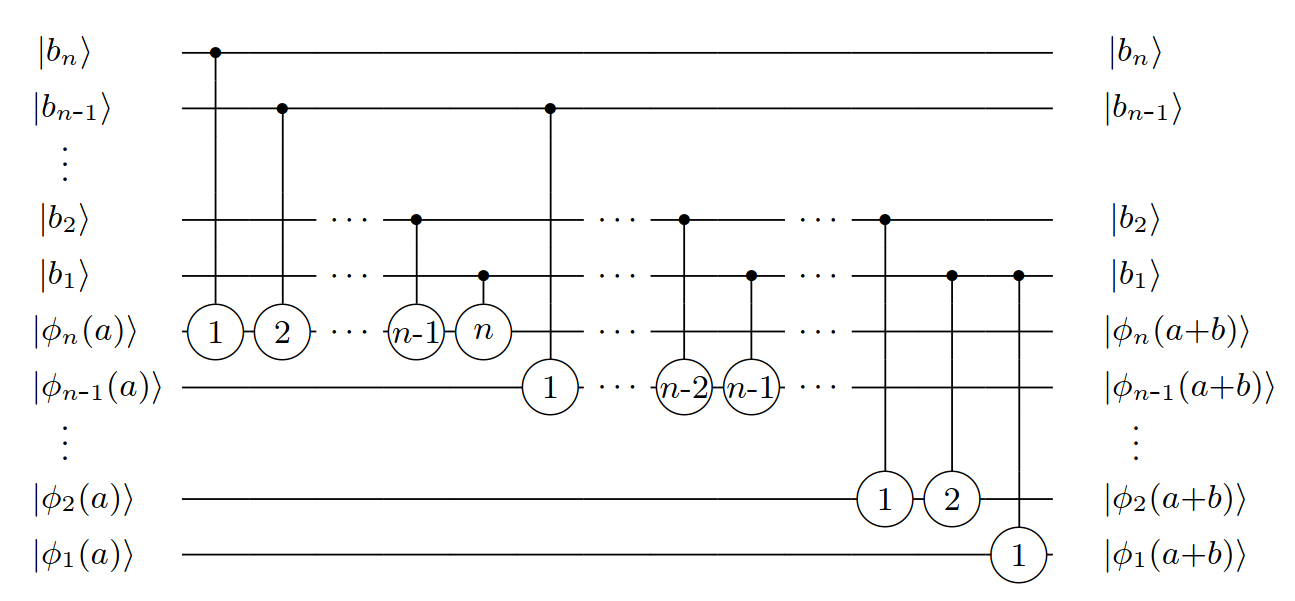
\includegraphics[width=\linewidth]{./draper.png}
	\end{figure}
\end{frame}

\begin{frame}{Tracing Draper's Adder}
	
	\begin{align*}
		\ket{\phi_n (a)}
		\xrightarrow{C_{b_n}-R_1}& 
		\frac{1}{\sqrt{2}} \Bigg(
		\ket{0} + \Big[  e(0.a_n a_{n-1} \cdots a_1) + e(0.b_n)\Big] \ket{1}
		\Bigg)\\
		\xrightarrow{C_{b_{n-1}}-R_2}& 
		\frac{1}{\sqrt{2}} \Bigg(
		\ket{0} + \Big[  e(0.a_n a_{n-1} \cdots a_1) + e(0.b_n b_{n-1})\Big] \ket{1}
		\Bigg)\\
		&\quad\quad\quad\quad\quad\vdots\\
		\xrightarrow{C_{b_1}-R_n}& 
		\frac{1}{\sqrt{2}} \Bigg(
			\ket{0} + \Big[  e(0.a_n a_{n-1} \cdots a_1) + e(0.b_n b_{n-1} \cdots b_1)\Big] \ket{1}
		\Bigg)\\
		&= \ket{\phi_n (a+b) }
	\end{align*}

\end{frame}


\begin{frame}{Parallel Adder}
	\begin{figure}[h]
		\centering
		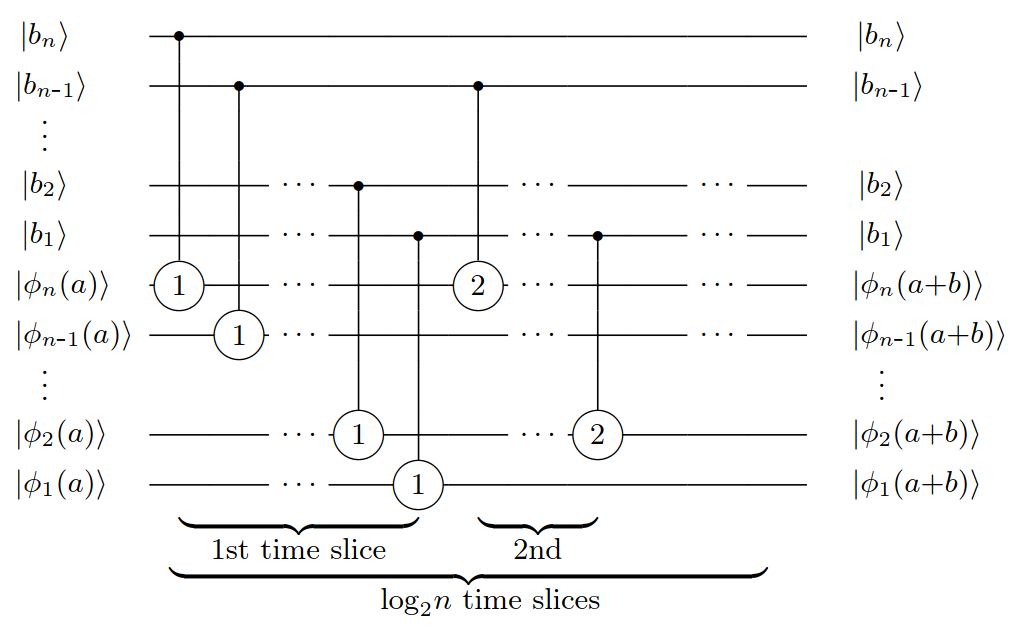
\includegraphics[width=\linewidth]{./paralleladder.png}
	\end{figure}
	
\end{frame}

\section{Beauregard's modular adder}%
\label{sec:beauregard_s_modular_adder}

\begin{frame}{Beauregard's Modular Adder}
	\begin{itemize}
		\item Use 2 controls (1 for $C-U_a$, 1 for building modular multipler).
		\item 1 ancilla qubit (must be cleared).
		\item Use one more qubit to store $a$ to prevent overflow and detect sign.
		\item Adding numbers larger than $N$ can be reduced.
	\end{itemize}
	
\end{frame}

\begin{frame}{Beauregard's Modular Adder}
	\begin{figure}[h]
		\centering
		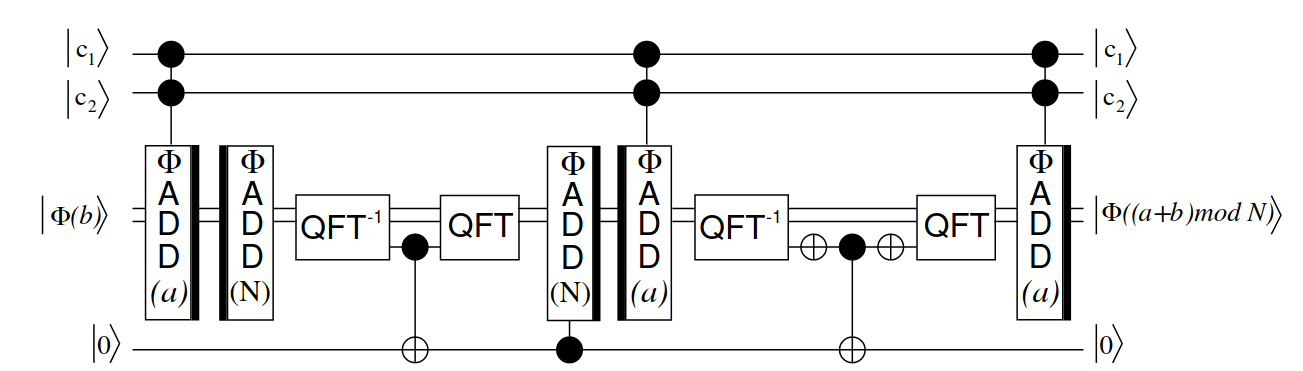
\includegraphics[width=\linewidth]{./beauregard_adder.png}
	\end{figure}
\end{frame}

\begin{frame}{Final Gate (for now)}
	\begin{figure}[h]
		\centering
		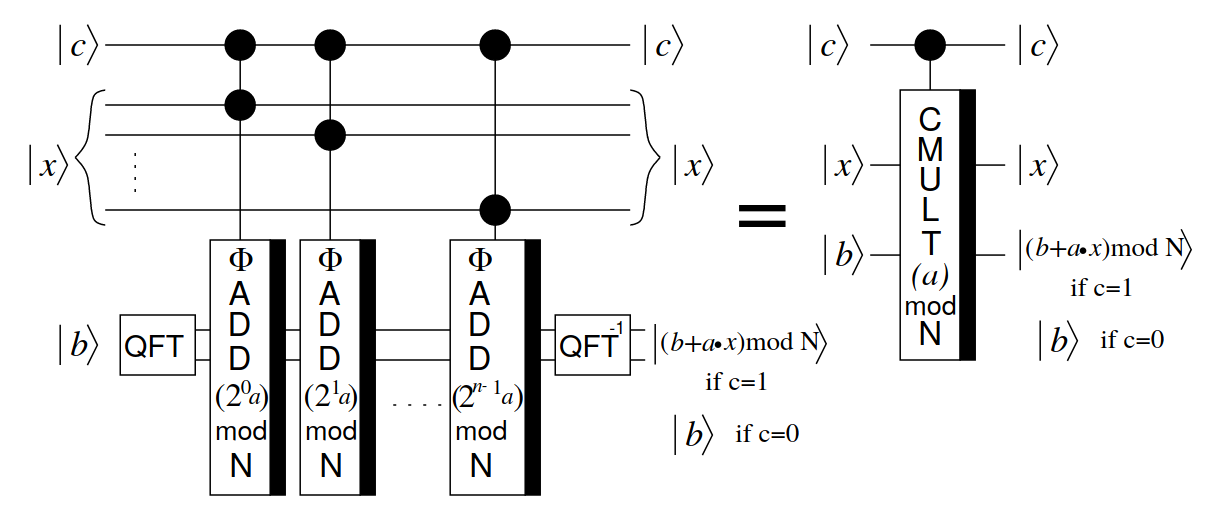
\includegraphics[width=\linewidth]{./ua.png}
	\end{figure}
\end{frame}

\section{Demonstration}%
\label{sec:demonstration}

\begin{frame}{title}
	
\end{frame}


\section{References}
\begin{frame}{References}
\begin{thebibliography}{10}
	\bibitem{pavlidis}Pavlidis, Archimedes, and Dimitris Gizopoulos. ``Fast
		Quantum Modular Exponentiation Architecture for Shor's Factorization
		Algorithm.'' \textit{arXiv preprint} arXiv:1207.0511 (2012). 
	\bibitem{draper}Draper, Thomas G. ``Addition on a quantum computer.'' 
		\textit{arXiv preprint} quant-ph/0008033 (2000). 
	\bibitem{beauregard}Beauregard, Stephane. ``Circuit for Shor's algorithm
		using 2n+ 3 qubits.'' \textit{arXiv preprint} quant-ph/0205095 (2002). 
	
\end{thebibliography}
\end{frame} 


\end{document}
